\documentclass[journal,onecolumn, draftclsnofoot, 12pt]{IEEEtran}
\usepackage[margin=1in]{geometry}
\usepackage[utf8]{inputenc}
\usepackage{graphicx}
\usepackage{times}
\usepackage{algorithm}
\usepackage{algpseudocode}
\usepackage{graphicx}
\usepackage{amsmath}
\usepackage{subcaption}
\usepackage{amsmath,amsfonts,amssymb,amsthm,commath,dsfont,enumitem}
\usepackage[colorlinks,urlcolor=blue,citecolor=blue]{hyperref}
\usepackage{xcolor}
\usepackage{listings}
\usepackage{todonotes}
\usepackage[T1]{fontenc}
\usepackage{graphicx} % for including the logo
\usepackage{fancyhdr} % for customizing the footer
\usepackage{tikz} % for the flowchart
\usetikzlibrary{shapes.geometric} % for tikz charts
\usetikzlibrary {arrows.meta,bending,positioning} % for tikz charts
\usepackage{array} % for R&V Tables
\usepackage{hyperref} % for hyper links

\pagestyle{fancy}

% % Define a new command to include a logo
% \newcommand{\logo}{\includegraphics[width=1.0cm]{OWB_cutout.png}}

% % Customize the footer to include the logo on the bottom right of pages 3 to 5
% \fancyfoot[LO,RE]{\ifnum\value{page}>3\ifnum\value{page}<19\logo\fi\fi}

% Setting color formatting for Python code
\lstset{
    language=Python,
    basicstyle=\fontsize{8}{10}\ttfamily,
    keywordstyle=\color{blue},
    stringstyle=\color{red},
    commentstyle=\color{green},
    morecomment=[l][\color{magenta}]{\#},
}

% Setting color formatting for C code
\lstset{
    language=C,
    basicstyle=\fontsize{8}{10}\ttfamily,
    keywordstyle=\color{blue},
    stringstyle=\color{red},
    commentstyle=\color{green!50!black},
    morecomment=[l][\color{magenta}]{\#},
    frame=tb,
    numbers=left,
    numberstyle=\tiny\color{gray},
    breaklines=true,
    showstringspaces=false,
}

% macros adapted from matus & djhsu
\def\ddefloop#1{\ifx\ddefloop#1\else\ddef{#1}\expandafter\ddefloop\fi}
\def\ddef#1{\expandafter\def\csname bb#1\endcsname{\ensuremath{\mathbb{#1}}}}
\ddefloop ABCDEFGHIJKLMNOPQRSTUVWXYZ\ddefloop
\def\ddef#1{\expandafter\def\csname b#1\endcsname{\ensuremath{\mathbf{#1}}}}
\ddefloop ABCDEFGHIJKLMNOPQRSTUVWXYZ\ddefloop
\def\ddef#1{\expandafter\def\csname c#1\endcsname{\ensuremath{\mathcal{#1}}}}
\ddefloop ABCDEFGHIJKLMNOPQRSTUVWXYZ\ddefloop

\DeclareMathOperator*{\argmin}{arg\,min}
\DeclareMathOperator*{\argmax}{arg\,max}
\DeclareMathOperator*{\softmax}{softmax}

\newenvironment{Q}{\item}{\phantom{s}}
\newenvironment{Solution}{\color{blue}\begin{enumerate}}{\end{enumerate}}

\begin{document}
\maketitle

\begin{titlepage}
    \begin{center}
        \vspace*{1cm}
            
        \Huge
        \textbf{ECE 445 Design Document - Spring 2024}
            
        \vspace{0.5cm}
        \LARGE
        OXYGEN DELIVERY ROBOT
            
        \vspace{1.5cm}

        \large
        Team \#27 \\
        Rutvik Sayankar \\ Aidan Dunican \\ Nazar Kalyniouk \\

        \vspace{1cm}
        
        TA: Selva Subramaniam

        \vspace{1.5cm}
            
        \vfill

        \vspace{0.8cm}
            
        \Large
        February 22nd, 2024 \\
        ECE 445: Senior Design Project Lab \\
        University of Illinois at Urbana-Champaign\\
            
    \end{center}
\end{titlepage}

\pagebreak

\tableofcontents

\pagebreak

\section{Terms and Keywords}
\vspace{0.8cm}
\begin{itemize}
    \item ChILD - Children's Interstitial and Diffuse Lung Disease
    \item PCB – Printed Circuit Board
    \item OWB - Three-Wheeled Omni-Wheel Bot
    \item UWB - Ultra-wideband is a radio technology that can use a very low energy level for short-range, high-bandwidth communications over a large portion of the radio spectrum.
    \item ESP32 - A series of low-cost, low-power system-on-a-chip microcontrollers with integrated Wi-Fi and dual-mode Bluetooth.
    \item RPM - Revolutions per minute
    \item GPIO - General-purpose input/output
    \item PWM - Pulse-width modulation
    \item MPH - Miles per hour
    \item OpenCV - (Open Source Computer Vision Library) is an open source computer vision and machine learning software library.
    \item OpenPose - Real-time multi-person keypoint detection library for body, face, hands, and foot estimation.
    \item TDoA - Time Difference of Arrival 
    \item ToF - Time of Flight
\end{itemize}

\pagebreak

\section{Introduction}

\subsection{Problem}
Children's interstitial and diffuse lung disease (ChILD) is a collection of diseases or disorders. These diseases cause a thickening of the interstitium (the tissue that extends throughout the lungs) due to scarring, inflammation, or fluid buildup \cite{ChILD-2022}. This eventually affects a patient’s ability to breathe and distribute enough oxygen to the blood.

Numerous children experience the impact of this situation, requiring supplemental oxygen for their daily activities. It hampers the mobility and freedom of young infants, diminishing their growth and confidence. Moreover, parents face an increased burden, not only caring for their child but also having to be directly involved in managing the oxygen tank as their child moves around.

\subsection{Solution}
Given the absence of relevant solutions in the current market, our project aims to ease the challenges faced by parents and provide the freedom for young children to explore their surroundings. As a proof of concept for an affordable solution, we propose a three-wheeled omnidirectional mobile robot capable of supporting filled oxygen tanks in the size range of M-2 to M-9, weighing 2.2 - 13.2 lbs (1 - 6kg) respectively (when full). Due to time constraints in the class and the objective to demonstrate the feasibility of a low-cost device, we plan to construct the robot at a roughly 50 percent scale of the proposed solution. Consequently, our robot will handle simulated weights/tanks with weights ranging from 1.1 - 6.6 lbs (0.5 - 3 kg). For our prototyping and testing, we will be utilizing an empty M-6 oxygen tank (height = 15", diameter = 3.2", empty weight = 2.8 lbs/1.27kg, capacity = 165L \cite{oxygen_tank_sizes}).

As mentioned the robot will have a three-wheeled omni-wheel drive train, incorporating two localization subsystems to ensure redundancy and enhance child safety. The first subsystem utilizes ultra-wide band (UWB) transceivers for triangulating the child's location relative to the robot in indoor environments, this is similar to how Apple AirTags triangulate their location relative to an iPhone \cite{airtag_uwb} (although AirTags use a combination of UWB and Bluetooth triangulation \cite{airtag_ble}). The second subsystem makes use of a desktop web camera which streams video to a Raspberry Pi where it will leverage open-source object tracking libraries to improve our directional accuracy in tracking a child. The final main subsystem focuses on the drive train and chassis of the robot.

As part of the design, we intend to create a PCB in the form of a Raspberry Pi hat, facilitating convenient access to information generated by our computer vision system, and saving space on our robot. The PCB will incorporate all motor control components, limit switch connections, GPIO pass through for the Raspberry Pi, power distribution and step down converter, and an STM32 based microcontroller serving as the project's central processing unit. This microcontroller will control the drivetrain, analyze UWB localization data, and use the direction vector provided by the computer vision system to calculate the speed and direction of each wheel.

\subsection{Visual Aid}

\begin{figure}[H]
\begin{center}
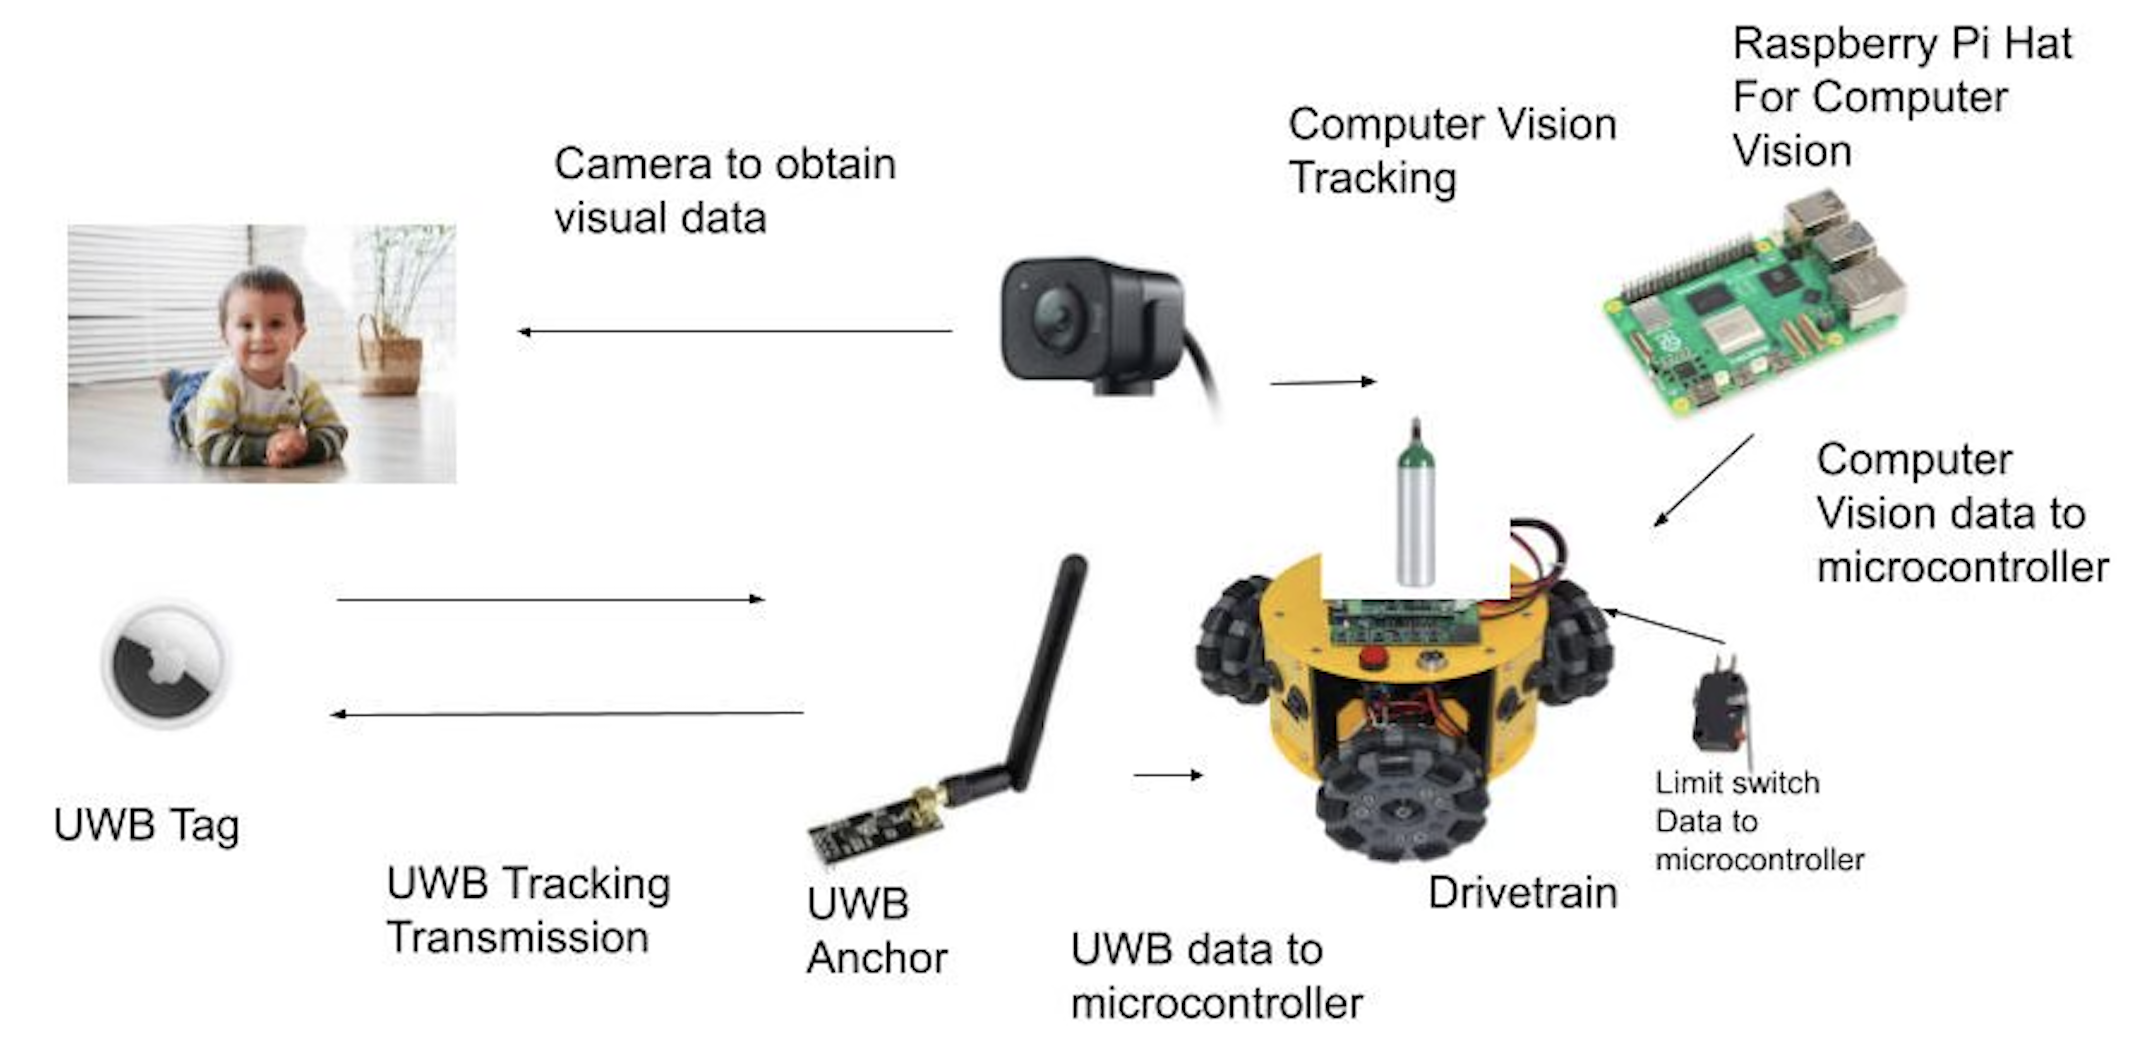
\includegraphics[width=0.9\textwidth]{VisualAid.png}\\
\caption{ Visual aid for our project.  } 
\label{fig:visualaid}
\end{center}
\end{figure}

\newpage

\subsection{High-Level Requirements List}
\begin{itemize}
    \item \textbf{Omni-wheel Drivetrain}: 
    The primary requisite pertains to the ability of the omni-wheel drivetrain to maintain heading according to a directional vector provided by our localization subsystems (UWB \& Computer Vision). This system will receive a the direction vector in the form of an array with broken down direction and speeds for each motor. Consequently, upon determination of a directional vector by our software, our robot is expected to initiate movement in the designated direction within 500 milliseconds.

    \item \textbf{UWB Localization}: 
    The subsequent criterion concerns the ability of the UWB localization system to produce precise positional data, with an accuracy threshold within 1 meter. We aim for continuous real-time updates regarding the child's whereabouts in relation to the robot.
    
    \item \textbf{Close-range Object Detection}: 
    The third requirement entails the implementation of close-range object detection mechanisms to discern obstacles obstructing the robot's trajectory. It is expected to promptly notify users of impending collisions, thereby safeguarding the child's well-being and facilitating timely intervention for obstacle removal.
    
\end{itemize}

\newpage

\section{Design}
\subsection{Block Diagrams}

\begin{figure}[H]
\begin{center}
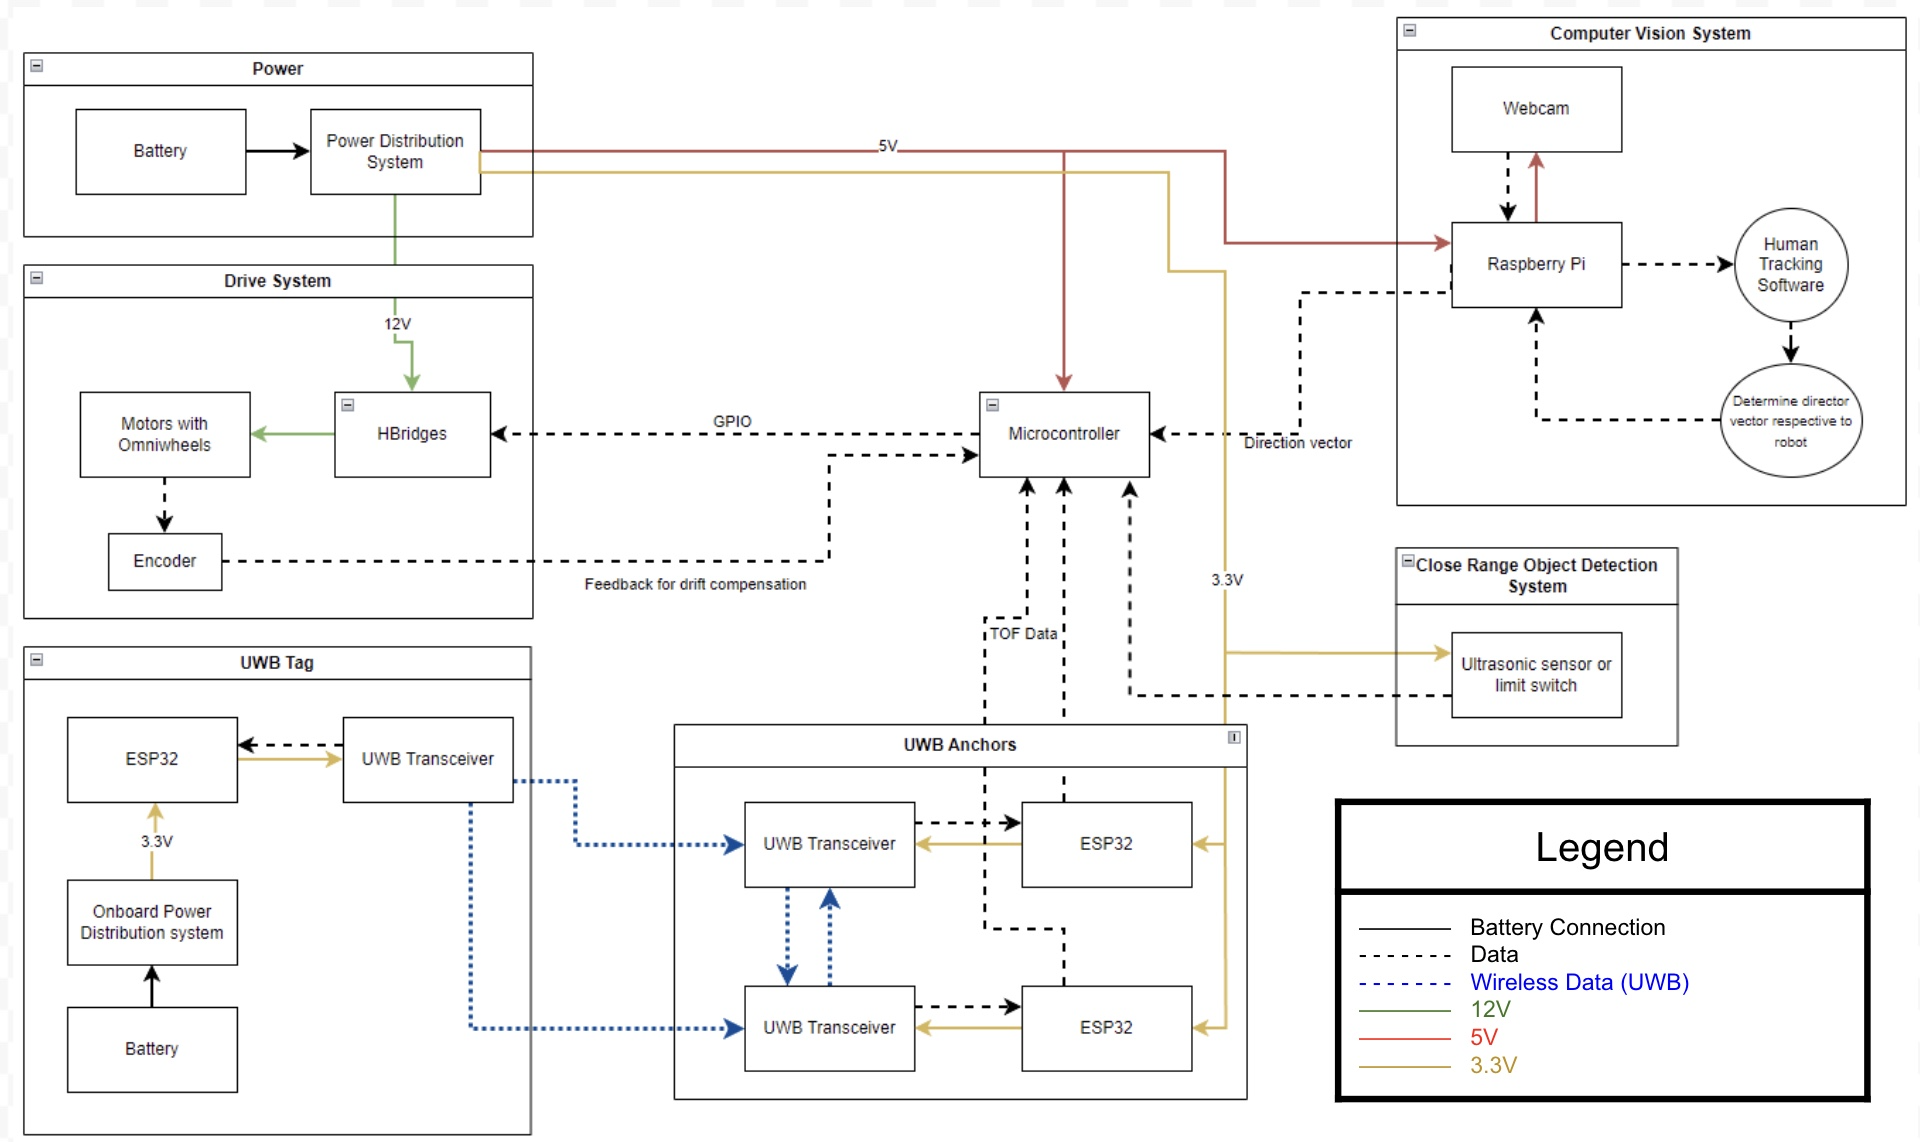
\includegraphics[width=1.0\textwidth]{BlockDiagram.png}\\
\caption{High-level block diagram for our project.  } 
\label{fig:blockdiagram}
\end{center}
\end{figure}


\subsection{Subsystems Overview}
\begin{itemize}
    \item \textbf{Drivetrain Subsystem}: The Drivetrain subsystem will encompass the motors, omni-wheels, encoder, and electronic speed controllers. It will receive instructions from the Control subsystem to control the motors and feed encoder data for drift compensation back to the Control subsystem (three-wheeled omni-wheel bots are easily affected by drift if it is not compensated for).
    \item \textbf{UWB Subsystem}: This subsystem contains tag and anchor components. The UWB tag will consist of the UWB transceiver, battery, ESP32, and onboard power distribution system. It will attach to the child that is being tracked (through velcro or some similar method). The UWB signals emitted are received by the UWB anchors. It will work with the UWB anchors subsystem to determine the location of the tag relative to the robot. The UWB anchors will consist of the UWB transceivers and ESP32s. This subsystem communicates with the Control Subsystem to relay a distance and angle that corresponds to the position of the tag relative to the anchors. Both of these systems will utilize transceiver boards based on Decawave DW3000 ICs \cite{9881375}.
    \item \textbf{Computer Vision Subsystem}: This subsystem will include a web camera connected to a Raspberry Pi. Implementing an image-processing algorithm using OpenCV or OpenPose it will analyze data from the web camera to locate the child. It will connect to the microprocessor and provide an angle. This angle will correspond to the change in angle required by the robot to keep the child within the center of the image frame (this will correspond to directly in front of the robot).
    \item \textbf{Close-Range Object Detection System}: This subsystem, consisting of bumper-style limit switches will communicate with the Control Subsystem to provide information about nearby obstacles. When an obstacle is detected (i.e. a limit switch has been activated), the user will be alerted to adjust the robot's path or clear the obstacle (through an LED or simple speaker). This feature will ensure effective obstacle avoidance and will enhance the safety of the robot.
    \item \textbf{Control and Power Subsystem}: The Control Subsystem will be responsible for taking in the distance and angle from the UWB Subsystem and the angle from the Computer Vision Subsystem. Facilitating a sensor fusion with this data, it will compute a velocity vector that the robot must move to remain within $\sim 1$ meter of the child. Using the kinematics detailed in section \ref{sec:OWBKinematics}, the velocity vector will be decomposed into its components to obtain the motor speed and direction for each omnidirectional wheel. 
    
    The Power Subsystem is responsible for supplying power to all other components of the robot. It will include a 12V battery and power distribution system. This subsystem will supply 12V power to the drive system. It will supply 5V to our STM32-based microcontroller, computer vision subsystem, and motor encoders. Lastly, it will supply 3.3V to the close-range object detection system and the UWB anchors.
\end{itemize}

\newpage

\subsection{Physical Design}
A rough idea of how everything will be put onto our robot is shown in figure \ref{fig:PhysicalDesign}.

\begin{figure}[H]
\begin{center}
    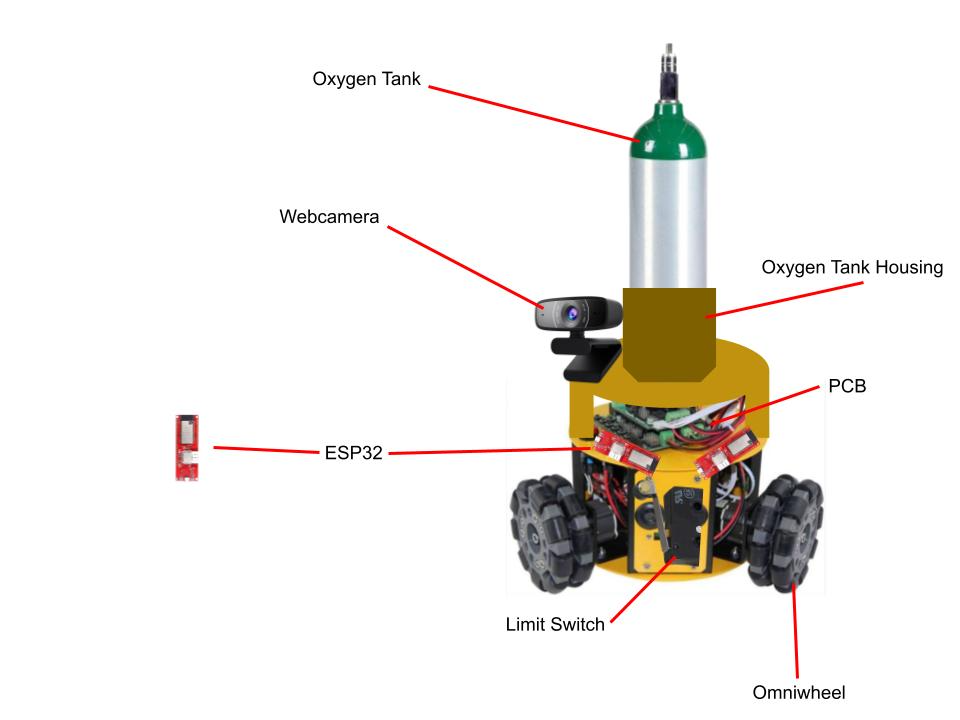
\includegraphics[width=0.8\textwidth]{PhysicalDesign.png}\\
    \caption{ Physical Layout  } 
    \label{fig:PhysicalDesign}
\end{center}
\end{figure}

\subsection{Drivetrain Subsystem}
This subsystem encapsulates everything required to move the chassis of the robot. To facilitate testing we will be using a RC Transmitter Controller which is detailed in section \ref{sec:RCController}. For more information regarding our choices of the commercial components that make up the Drivetrain Subsystem, please refer to section \ref{sec:cost}. Regarding the safety of our OWB, the Drivetrain Subsystem must accept commands from the Control Subsystem to set the relative speed of the motors.

\subsubsection{Kinematics of the OWB}
\label{sec:OWBKinematics}
In a three-wheeled omni-wheel robot, the three wheels are arranged in a triangular pattern, with one wheel at the front and two wheels at the back. Each wheel has several small omnidirectional wheels arranged in a circular pattern, which allows the robot to move in any direction.

To move the robot, each wheel is driven independently using a motor. By varying the speed and direction of each wheel, the robot can move in any direction and rotate around its center point.

The kinematics of a three-wheeled omni-wheel robot can be modeled mathematically through the below equations \cite{riky2021omnidirectional} which relate the robot's linear and angular velocities to the speed and direction of each wheel.

We first define for each wheel a direction of rotation $V_i$, and the resulting movement effected in the x and y axes, $V_ix$ and $V_iy$ as shown below.


\begin{figure}[H]
  \centering
  \begin{minipage}[b]{0.45\linewidth}
    \centering
    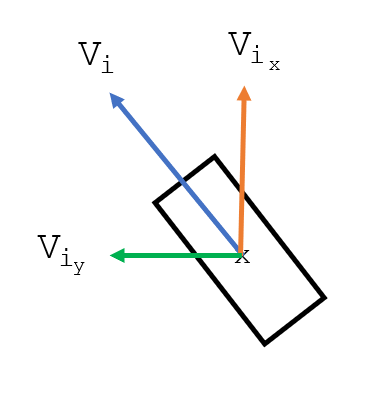
\includegraphics[width=\linewidth]{wheel_vector.png}
    \caption{Vector Definitions}
    \label{fig:vecdef}
  \end{minipage}
  \hfill
  \begin{minipage}[b]{0.45\linewidth}
    \centering
    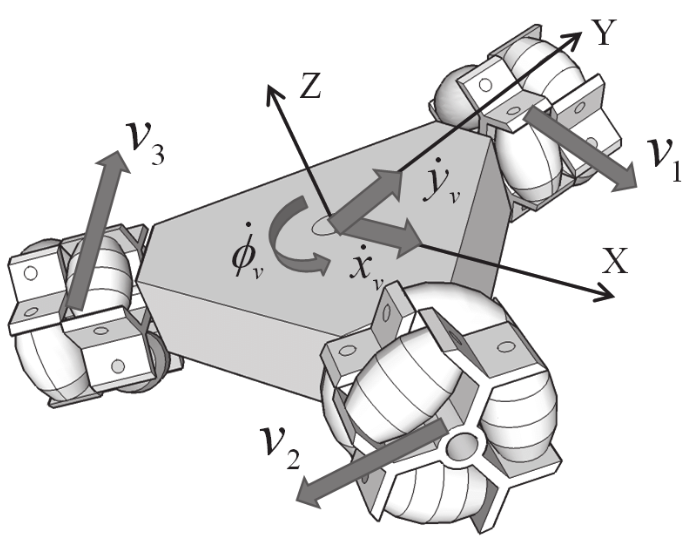
\includegraphics[width=\linewidth]{OWB_vectors.PNG}
    \caption{OWB drive vectors \cite{wada2015OWB}}
    \label{fig:owb_vec}
  \end{minipage}

  \label{fig:vecs}
\end{figure}

Knowing the angle of each wheel from the vertical axis, we can compute the x and y components created by the rotation of each wheel. By summing these components together, we can get the effective motion of the robot in the x, y and yaw axes.

\[
\begin{pmatrix}
V_x \\
V_y \\
\omega
\end{pmatrix}
=
\begin{pmatrix}
1 & - \frac{1}{2} & -\frac{1}{2} \\
0 & -\frac{\sqrt{3}}{2} & \frac{\sqrt{3}}{2} \\
1 & 1 & 1
\end{pmatrix}
\begin{pmatrix}
V_1 \\
V_2 \\
V_3
\end{pmatrix}
\]
    
$V_{x}$ and $V_{y}$ are the desired linear velocities in the x and y directions, respectively, and omega is the desired angular velocity. $V_{1}$, $V_{2}$, and $V_{3}$ are the velocities of the three wheels, and L is the distance between the robot's center of mass and the wheel axes.

\[
\begin{pmatrix}
V_1 \\
V_2 \\
V_3
\end{pmatrix}
=
\begin{pmatrix}
1 & - \frac{1}{2} & -\frac{1}{2} \\
0 & -\frac{\sqrt{3}}{2} & \frac{\sqrt{3}}{2} \\
1 & 1 & 1
\end{pmatrix}^{-1}
\begin{pmatrix}
V_x \\
V_y \\
\omega
\end{pmatrix}
\]

By taking the inverse of our 3x3 component coefficient matrix above, we can solve for our individual motor speeds $V_1$, $V_2$ and $V_3$, given the desired motion in terms of $V_x$, $V_y$, and $w$.


\subsubsection{Communication for RC Controller}
\label{sec:RCController}
For our RC controller, we plan to use a Flysky FS-i6 6CH 2.4GHz Radio System RC Transmitter Controller with FS-iA6 Receiver. 

This controller communicates with its receiver, the FS-iA6, using a 2.4 GHz digital frequency-hopping spread spectrum (FHSS) communication protocol.

In FHSS, the transmitter and receiver periodically hop between different channels within the 2.4 GHz frequency band to avoid interference from other devices operating on the same frequency band. The specific channels used are selected automatically by the transmitter and receiver and can be different for each transmission.

The FS-i6 transmitter sends digital signals to the FS-iA6 receiver, which is connected to the RC vehicle's onboard electronics. The transmitter and receiver are bound together before use, which pairs them and allows them to communicate securely.

The FS-i6 transmitter has six channels of control, which means it can transmit six different control signals to the receiver at the same time. These channels can be used to control the movement of the RC vehicle's motors and servos, as well as to operate other electronic components such as lights or sound systems.

For our operations, we plan to use three channels, using our OWB as our frame of reference, we used one channel for linear control in the $x-axis$ a second for linear control in the $y-axis$, and a third channel for rotational control $w$

The OWB can move forward and backward like a normal RC car. This motion is represented by $V_y$, and is mapped to CH1 on the transmitter (refer to figure \ref{fig:ChannelDistribution} for detail on channel mapping). While a normal RC car needs a $V_y$ component to turn left or right, the OWB can "yaw" on the spot. This is represented by $w$, and is mapped to CH3 on the transmitter. The final unique motion the OWB can execute is a "drift" toward the left or right. This motion is represented by $V_x$ and is mapped to CH2 on the transmitter.

Thus, using these three channels, we can define the robot's desired $V_x$, $V_y$, and $w$. These desired motion vectors are then fed to our inverse kinematics algorithm, which breaks down our desired motion into an individual wheel speed and direction for each motor.

\begin{figure}[H]
\begin{center}
    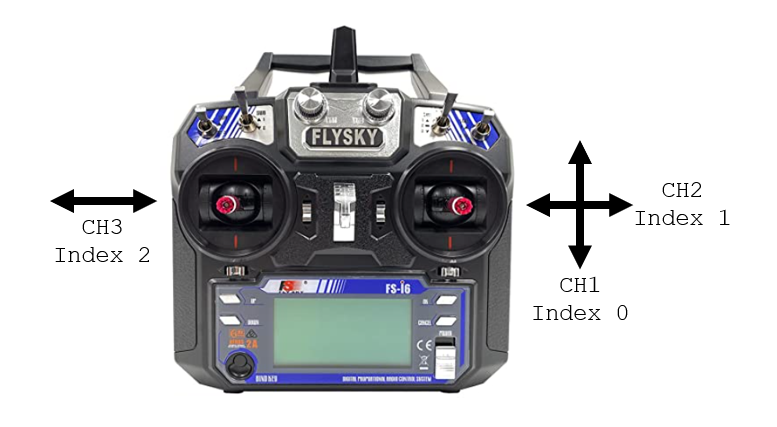
\includegraphics[width=0.8\textwidth]{channel.png}\\
    \caption{ Channel Distribution  } 
    \label{fig:ChannelDistribution}
\end{center}
\end{figure}

\newpage

\subsubsection{Requirements and Verification}
\begin{center}
\begin{tabular}{ | m{20em} || m{20em} | } 
  \hline
  Requirements & Verification  \\ 
  \hline
  \hline
  The electronic speed controllers power the motors at the command of the board control subsystem. The commands may be to set duty cycle, set current, or set RPM. 
  & 
  Ensure the OWB is at an idle state such that the wheels are not spinning. Then, send a command to both ESCs from the board microcontroller to either set a nonzero duty cycle, current, or RPM. Confirm that both motors begin spinning.
  \\ 
  \hline
  The drivetrain must be able to maintain a speed of at least 3 MPH (that fastest speed we are comfortable following a user), with a fully loaded oxygen tank (Full tank at 3.458 lbs + roughly 10 lbs of chassis, electronics, battery weight).
  & 
  Ensure the OWB is at an idle state such that the wheels are not spinning. Load the oxygen tank onto the robot and add any extra weight to help simulate a full oxygen tank. 
  
  Set up a specific distance for the robot to drive. Using a stopwatch, time the robot as it travels the specified distance.
  
  Using an external RC controller drive the robot forward until it passes the specified distance.
  
  Using the time measurement and the specified distance, measure the speed and ensure it is > 3 MPH.
  \\
  \hline
\end{tabular}
\end{center}

\vspace{0.8cm}

\subsection{UWB Subsystem}
This subsystem encapsulates everything required to obtain a direction and angle of the UWB Tag relative to the UWB Anchors. It will transmit these values to the Control Subsystem. To facilitate the testing of our localization algorithm we will use the indoor positioning visualization example provided by MakerFabs (\url{https://github.com/Makerfabs/Makerfabs-ESP32-UWB.git}). There are two steps to our localization algorithm that are detailed in section \ref{sec:Localization}. For more information regarding our choices of the commercial components that make up the UWB Subsystem, please refer to section \ref{sec:cost}.

\vspace{0.5cm}

\subsubsection{Localization Algorithms}
\label{sec:Localization}

There are two main localization techniques when we use UWB, Time Difference of Arrival (TDoA) and Time of Flight (ToF) \cite{localization}.

ToF is a positioning method based on two-way ranging. That means the tag needs to send and receive signals from the anchor several times and then the flight time of the signal between the anchor and the tag can be measured, because radio waves travel at the speed of light, we can calculate the distance between the tag and each anchor.

TDoA is localization based on comparing the time difference between signals and each anchor and this technique requires an accurate time synchronization function. When using the TDoA method, the UWB tag will send out a poll message, and all the nearby UWB anchors will receive it and record the arrival time. Because the location of anchors is different, they won’t receive the message at the same time. We can use these time differences to determine the tag’s location.

This algorithm will essentially provide us with the sides of a triangle, with which we can calculate the location of the tag, we will be using the law of cosines to triangulate the location of the tag relative to the anchors.

\begin{algorithm}[H]
    \SetAlgoLined
    
    \Input{\textbf{Input}: Lengths of sides $(a, b, c)$}\\
    \Output{\textbf{Output}: Coordinates $(x, y)$} 

    % cos_a = (b * b + c*c - a * a) / (2 * b * c)
    % x = b * cos_a
    % y = b * cmath.sqrt(1 - cos_a * cos_a)
    
    $ \text{cos\_a} = \frac{{b^2 + c^2 - a^2}}{{2bc}} $\; \\
    $ x = b \cdot \text{cos\_a} $\; \\
    $ y = b \cdot \sqrt{1 - \text{cos\_a}^2} $\; \\
    
    \Return{$ (\text{round}(x.\text{real}, 1), \text{round}(y.\text{real}, 1)) $}\;
    
    \caption{Calculation of Coordinates using Law of Cosines}
\end{algorithm}

\newpage

\subsubsection{Requirements and Verification}
\begin{center}
\begin{tabular}{ | m{20em} || m{20em} | } 
  \hline
  Requirements & Verification  \\ 
  \hline
  \hline
  Utilize ToF or TDoA localization to create a triangle of known lengths with vertices defined by each UWB transceiver.
  & 
  Ensure the OWB is at an idle state such that the wheels are not spinning. Then, place the UWB Tag one meter away from the robot. Utilizing the visualization program by MakerFabs, we will test our algorithm by comparing the location that was calculated for the tag with the real-world location. Confirm that the proper location is displayed.
  \\ 
  \hline
\end{tabular}
\end{center}

\subsection{Computer Vision Subsystem}
This subsystem encapsulates everything required to obtain the angle of the child relative to the OWB. It will transmit this value to the Control Subsystem. To facilitate the testing of this subsystem we will connect our Raspberry Pi to monitor in order to ensure that we are properly locating and tracking the child. For more information regarding our choices of the commercial components that make up the Computer Vision Subsystem, please refer to section \ref{sec:cost}.

\vspace{0.5cm}

\subsubsection{OpenCV Algorithms}
The code will load a pre-trained Haar cascade classifier specifically designed for detecting full-body patterns, which will assist in identifying individuals within images.
 
When a child is detected within the image, the algorithm analyzes their position. This involves calculating the center point of the detected child's body and determining the relative distance between this center point and the center of the entire image.
 
The algorithm calculates center points and the relative distance. A variable called "Degrees Off Center" will be calculated by finding the differences between both center points. If this value is greater than 9\%, then a correction will be made. The calculation for this value can be found in section \ref{sec:anglecalc}.


\newpage

\begin{figure}[h]
    \centering
    \begin{tikzpicture}[node distance=2cm, shift={(-5, -10)}, scale=0.25]
        % Define nodes
        \node at (-5cm,0) (Camera) [circle, draw, xshift=-3cm] {\begin{minipage}{2cm} \centering
            Logitech Camera \\
            Input
          \end{minipage}};
        \node (Check) [diamond, draw, below of=Camera, yshift=-2cm, scale=0.8] {\begin{minipage}{3cm} \centering
            Image Captured \\
            Successfully by \\ Raspberry Pi
          \end{minipage}};
        \node (Objectdet) [rectangle, draw, below of=Check, yshift=-1cm] {Preform Object Detection};
        \node (Percent) [rectangle, draw, below of=Objectdet] {\begin{minipage}{3cm} \centering Perecent of \\ Screen Algorithm\end{minipage}};
        \node (EndDet) [rectangle, draw, left of=Check, xshift=-4cm] {Image Detection Ended};
        \node (Correc) [rectangle, draw, below of=Percent] {Preform Correction};
        \node (Send) [rectangle, draw, left of=Correc, xshift=-2cm] {Send To STM};
    
        % Define edges
        \draw [->] (Camera) -- node[right]{USB} (Check);
        \draw [->] (Check) -- node[right]{Yes} (Objectdet);
        \draw [->] (Objectdet) -- node[above]{} (Percent);
        \draw [->] (Check) -- node[above]{No} (EndDet);
        \draw [->] (Percent) -- node[right]{if $\geq 9\%$} (Correc);
        \draw [draw = thick,
         arrows={
         - 
           Stealth[length=8pt,open,bend,sep]}] (Correc) edge [bend right=95] (Objectdet);
        \draw [->] (Correc) -- (Send);
        
        

    \end{tikzpicture}
    \caption{Angle Correction Feedback Loop Flowchart}
    \label{fig:flowchart}
\end{figure}

\newpage

\subsubsection{Requirements and Verification}
\begin{center}
\begin{tabular}{ | m{20em} || m{20em} | } 
  \hline
  Requirements & Verification  \\ 
  \hline
  \hline
  Utilize OpenCV or OpenPose to determine $\Delta \theta$ of the child respective to the center of the robot.
  & 
  Ensure the OWB is at an idle state such that the wheels are not spinning. Then, stand slightly off-center from the front of the robot. While having the Raspberry Pi plugged into the monitor, display the video feed with overlayed boxes for the tracked object. Using an additional overlay on the video, there should be an angle that defines the degrees from the center of our target. Compared with the measured value.
  \\ 
  \hline
\end{tabular}
\end{center}

\subsection{Close-Range Object Detection System}
This subsystem encapsulates everything required to detect objects directly within the robot's path of travel. Upon activation of bumper-style limit switches on all sides of the robot, a signal will be sent to the Control Subsystem which will deactivate the motors and trigger an alert system. For more information regarding our choices of the commercial components that make up the Close-Range Object Detection Subsystem, please refer to section \ref{sec:cost}.

\subsubsection{Requirements and Verification}
\begin{center}
\begin{tabular}{ | m{20em} || m{20em} | } 
  \hline
  Requirements & Verification  \\ 
  \hline
  \hline
  The bumper-style limit switch should trigger an alert system and stop all motors until the bumper is depressed.
  & 
  Ensure the OWB is at an idle state such that the wheels are not spinning. Then, move the UWB tag such that the Robot must move to compensate for the change in the Tag's location. During the robot's travel, trigger one of the limit switches. The robot should stop and the alert system should trigger.
  \\ 
  \hline
\end{tabular}
\end{center}

\subsection{Control and Power Subsystem}
This subsystem encapsulates our main microcontroller and all power step-down converters to supply power to the individual components at the required levels. 

The Control subsystem will take in direction and angle vectors from the UWB Subsystem, and angle from Computer Vision Subsystem. We will then perform a sensor fusion where we place greater weight on the data provided by the UWB Subsystem, and allow for minor corrections through the Computer Vision Subsystem. This system will then decompose the direction and angles to obtain a direction vector which will be decomposed into individual wheel speeds as detailed in section \ref{sec:OWBKinematics}.

The Power Subsystem is responsible for supplying power to all other components of the robot. It will include a 12V battery and power distribution system. This subsystem will supply 12V power to the drive system. It will supply 5V to our STM32-based microcontroller, computer vision subsystem, and motor encoders. Lastly, it will supply 3.3V to the close-range object detection system and the UWB anchors. Refer to figure \ref{fig:Buck_12_5} for a calculation on stepping down from 12V to 5V and figure \ref{fig:Buck_12_3} for a calculation on stepping down from 12V to 3.3V.

\begin{figure}[H]
\begin{center}
    \includegraphics[width=0.8\textwidth]{BuckConverter12_5.png}\\
    \caption{ Buck Converter Sizing 12V to 5V  } 
    \label{fig:Buck_12_5}
\end{center}
\end{figure}

\begin{figure}[H]
\begin{center}
    \includegraphics[width=0.8\textwidth]{BuckConverter_12_3.png}\\
    \caption{ Buck Converter Sizing 12V to 3.3V  } 
    \label{fig:Buck_12_3}
\end{center}
\end{figure}


\subsubsection{Requirements and Verification}
\begin{center}
\begin{tabular}{ | m{20em} || m{20em} | } 
  \hline
  Requirements & Verification  \\ 
  \hline
  \hline
  Control Subsystem: Using the direction and angle vectors from the UWB Subsystem, and angle from Computer Vision Subsystem we should compute a direction vector for the robot to move.
  & 
  Connecting a serial output to our STM32, we should be able to read a direction vector in the frame of reference of our robot. Compare it to the location of the UWB Tag.
  \\ 
  \hline
  Power Subsystem: Must be able to regulate battery voltage to power components throughout the discharge cycle of the battery and automatically cut out power when battery voltage drops too low.
  & 
  Connect the input of the voltage regulator to the voltage supply. Connect the output of the voltage regulator to a programmable load. Set voltage supply to maximum battery voltage.
  
  Check the voltage reading with a multimeter to make sure the output voltage does not fall outside of 12V $\pm$ 5\% under no load and full load. 
  \\ 
  \hline
\end{tabular}
\end{center}

\newpage

\subsection{OpenCV Supporting Material}

Figure \ref{fig:CVModule_PerformanceTest} has a sample image of a child as well as the vertical lines at the two center points. In this scenario, a corrective measure will need to be taken since the child is too far off the center of the screen.

\begin{figure}[H]
\begin{center}
    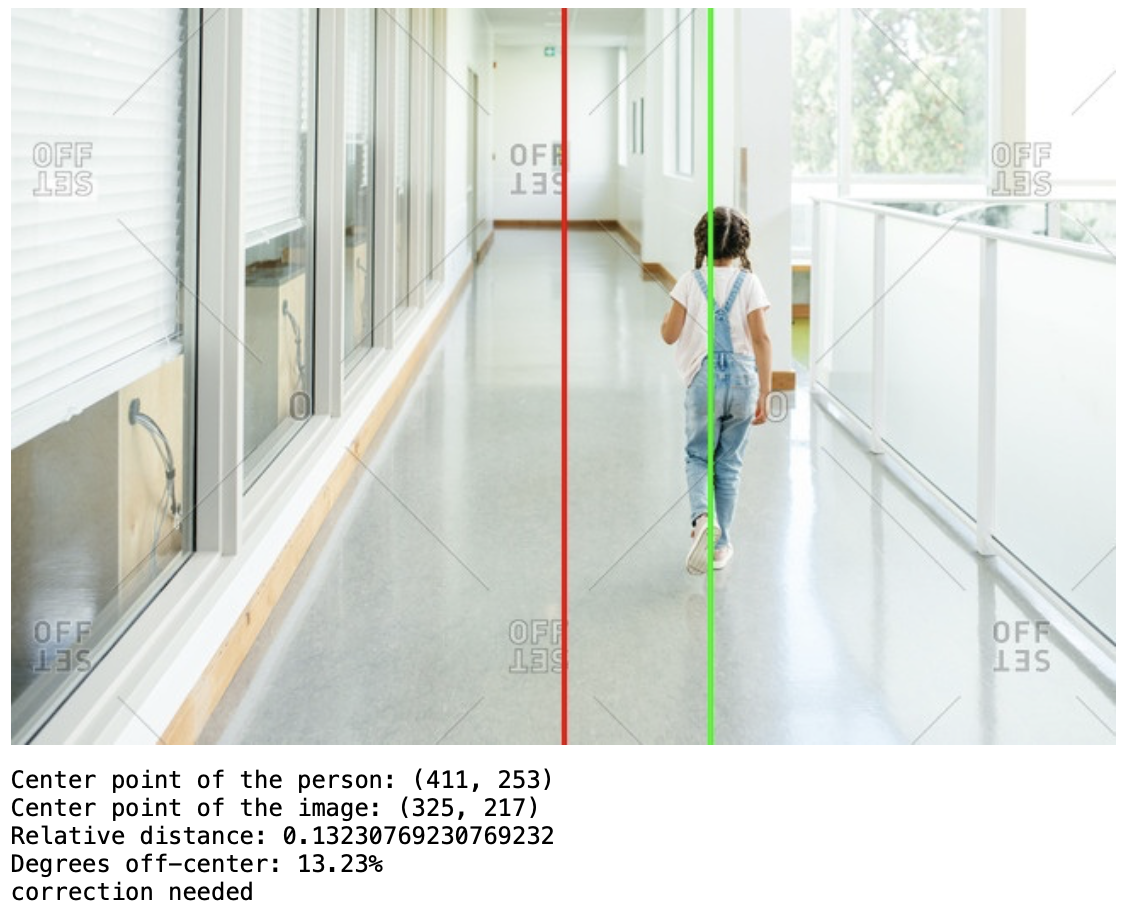
\includegraphics[width=0.7\textwidth]{CVModule_PerformanceTest.png}\\
    \caption{ OpenCV Performance Test  } 
    \label{fig:CVModule_PerformanceTest}
\end{center}
\end{figure}

The provided code in figure \ref{fig:CVModule_TestCode} uses OpenCV to detect bodies in an input image using a pre-trained Haar cascade classifier. If bodies are detected, it calculates the distance of the center of the detected body from the center of the image. Vertical lines are drawn at the center of the child and the center of the screen. A relative distance is calculated by subtracting the two center points and dividing that value by the number of pixels of the screen. This provides the degrees-off-center value and will print a message if a correction is required. In testing, this value can be adjusted later. If no person is detected, it prints a message indicating so.

\begin{figure}[H]
\begin{center}
    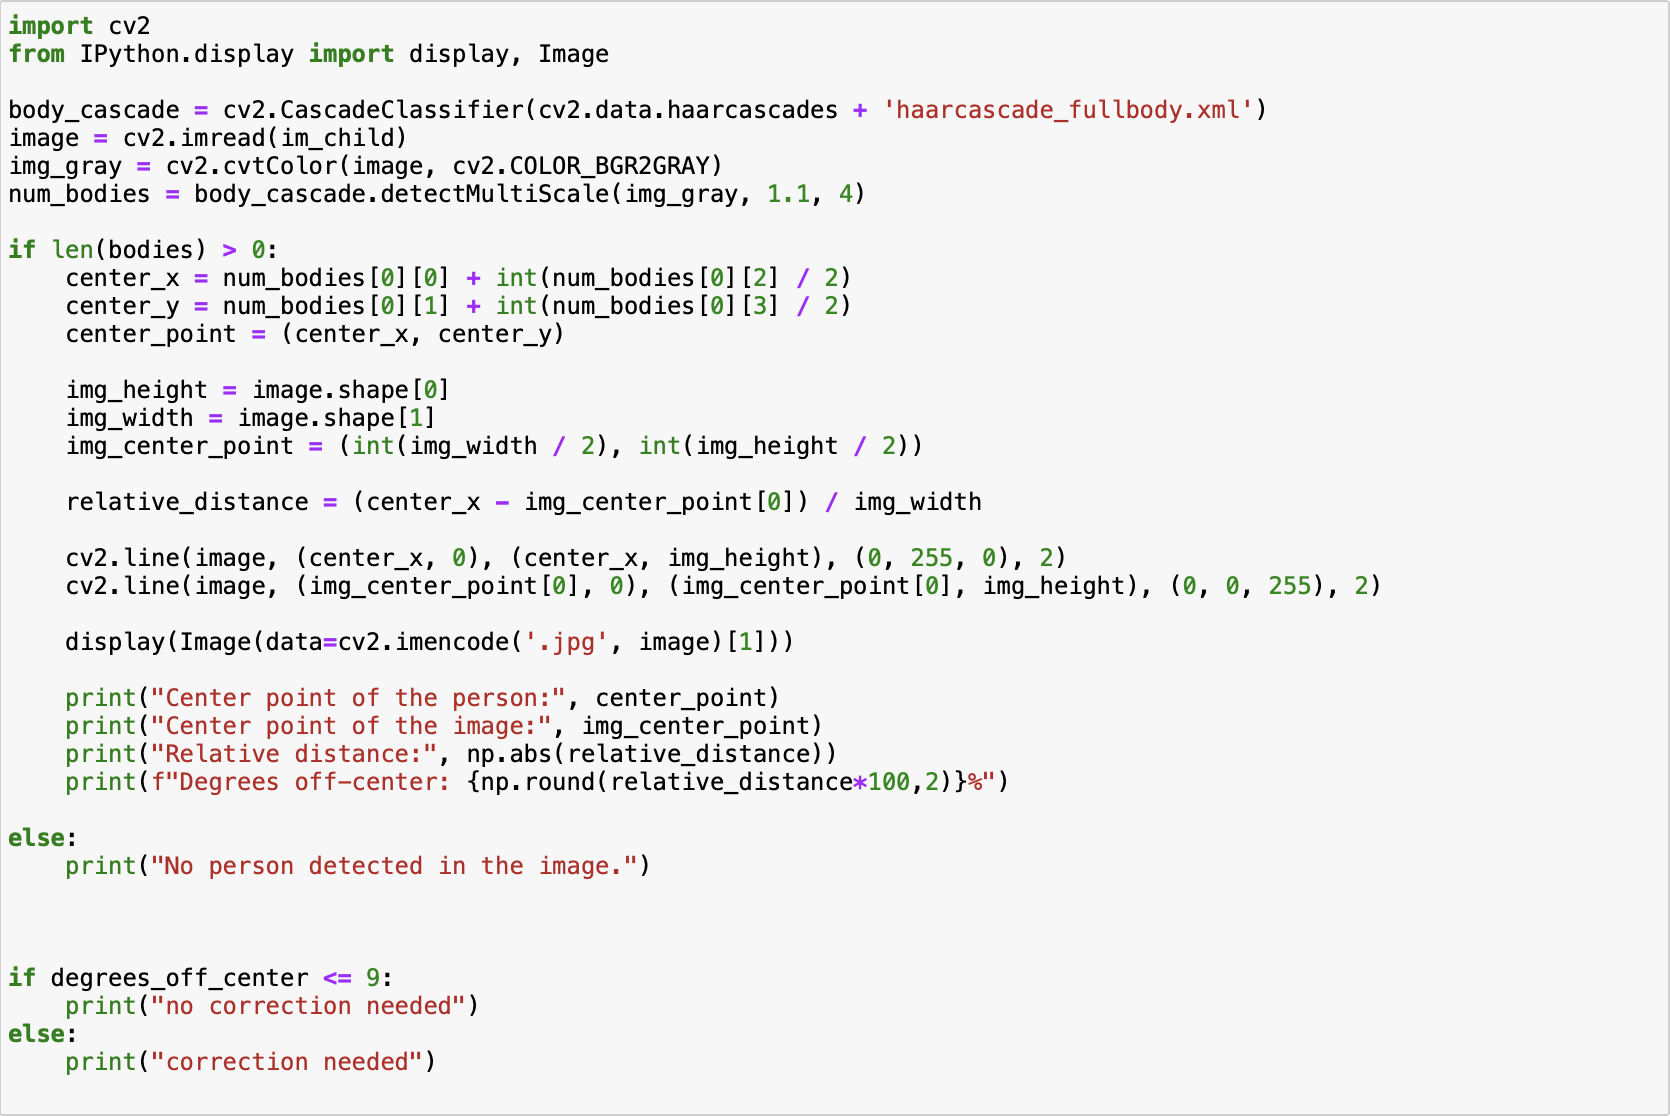
\includegraphics[width=0.7\textwidth]{CVModule_TestCode.png}\\
    \caption{ OpenCV Test Code  } 
    \label{fig:CVModule_TestCode}
\end{center}
\end{figure}


\subsection{Tolerance Analysis}

\subsubsection{Computer Vision Angle Analysis}\;\\
\label{sec:anglecalc}
Average Shoulder Width of Child = 9 in. = 0.23 m. \\
Resolution of Camera = 1600 x 1200 pixels \\
FOV of Camera = 75 degrees \\
\\
The child will be a distance of 1 m. $\pm$ 25\% (0.75 m. -- 1.25 m.) away from the robot. Figure \ref{fig:calc2} is an image of the minimum and maximum ranges. The red boxes are used to represent the width of the child. 
To calculate how much of the screen the child will take up, we must first calculate the horizontal width of the FOV. This is done by performing some simple trigonometry. The calculation for 1 meter will be done below. The same process will be done for 0.75 meters and 1.25 meters. \\

\begin{figure}[H]
\begin{center}
    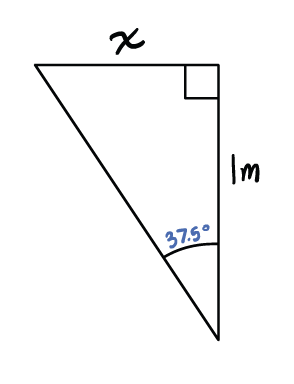
\includegraphics[width=0.3\textwidth]{calc1.png}\\
    \caption{Calculation of Horizonatal FOV width} 
    \label{fig:calc1}
\end{center}
\end{figure}

Half of FOV = \( \frac{75^\circ}{2} = 37.5^\circ \) \\
 
$x = (1 \text{ meter}) \times \tan(37.5^\circ) = 0.767 \text{ meters}$ \\
Now, we multiply this distance by 2, and we get the horizontal FOV width.
Horizontal FOV Width = $0.767 \text{ meters} \times 2 = 1.534 \text{ meters}$ 
Take the average shoulder width of the child and divide it the value you just found.
Percent of Screen = $\frac{\text{Average Shoulder Width of Child}}{\text{Horizontal FOV Width}} = 15\%$
A diagram with the calculated percentages can be found in figure \ref{fig:calc2}.

\begin{figure}[H]
\begin{center}
    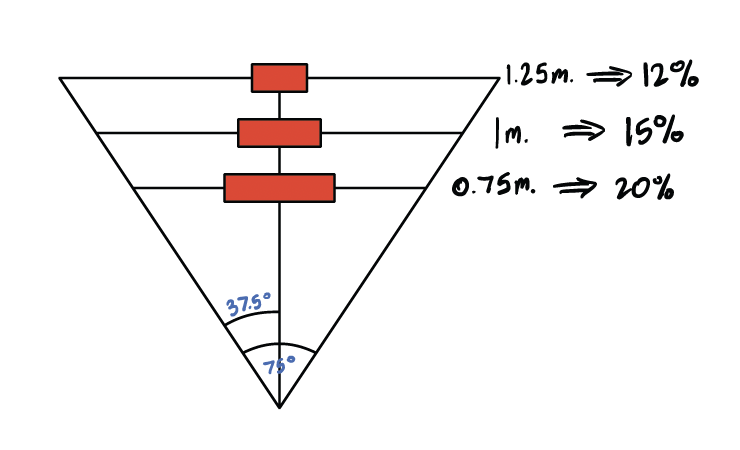
\includegraphics[width=0.8\textwidth]{calc2.png}\\
    \caption{Percent of screen calculations for openCV algorithm} 
    \label{fig:calc2}
\end{center}
\end{figure}
 
Since we want to stay within this range, the tolerance for the Percent of Screen taken up by the child will be \(15\% \pm 3\%\). 
The center of the child and the center of the screen will be compared to determine if a correction will be made. Therefore, we divide \( 15\% \) by \( 2\% \) to get \( 7.5\% \) and add \( 1.5\% \) to that value, so if the difference between the two midpoints is more than \( 9\% \), then a correction will be made.

\subsection{Risk Analysis}

Robots and oxygen tanks are both inherently dangerous as they stand and combining the two together carries additional risks to the user and people around them. Since our project is meant to assist young children in their daily lives, we must take extra precautions in order to ensure their safety. When designing the subsystems, there are two we aim to focus on in order to provide the appropriate safety features required for our project. One of the main concerns that we must address is in regard to the oxygen tank we wish to have driven around by our robot. To reduce the risk of injury from the oxygen tank, we plan to design a bottom heavy and wide base to our robot to prevent the tipping hazard. In addition, during design and testing, our oxygen tank will be empty in order to ensure that no accidental release of pressure can occur. Since our robot is carrying the tank, we will also focus heavily on our microcontroller to provide a bulk of the safety features. To reduce this risk of injury, we will incorporate the following safety principles into our design. If the UWB connection and or Computer Vision connection fail, our microcontroller will safely disengage all of the motors entirely. This disengagement of the motors will need to be gradual as sudden braking of the robot can cause the robot to tip over and cause severe injury. Our microcontroller will be tasked with limiting the speed to the robot to speeds of less than 3 mph to ensure no injury will occur. Finally, we will include limit switches in the form of a bumper around the perimeter of our robot to ensure that the robot will come to a complete stop when it encounters an object in the way of its path, whether that object is the patient or some other external debris. In short, we will attempt to mitigate the primary safety concerns associated with utilizing oxygen tanks and failures that may occur in our subsystems that are responsible for giving inputs to our motors. 

\section{Cost and Schedule}
\label{sec:cost}

\subsection{Cost Analysis}
The cost for parts has been derived from figure \ref{fig:ComponentCost}. Before shipping our project cost is \$665.31. Estimated shipping cost will be 5\%, which will add another \$33.27 and with a sales tax of 10\%, another \$66.53 will be added. We can expect a salary of \$42/hr $\times$ 2.5 hr $\times$ 60 hours to complete = \$6300 per team member. We need to multiply this amount with the number of team members, \$6300 $\times$ 3 = \$18,900 in labor cost. This comes out to be a total cost of \$19,665.11.

\begin{figure}[H]
\begin{center}
\begin{tabular}{ | m{10em} || m{10em} || m{10em} || m{5em} | } 
  \hline
  Item & Manufacturer & Quantity & Cost  \\ 
  \hline
  \hline
  \href{https://www.gobilda.com/modern-robotics-12vdc-motor/}{12VDC motors}
  &
  Modern Robotics
  &
  3
  &
  14.99
  \\
  \hline
  \href{https://www.pitsco.com/TETRIX-Omni-Wheel-Packs?SKU=}{Omni Wheel Packs}
  &
  TETRIX MAX
  &
  3
  &
  29.95
  \\
  \hline
  \href{https://www.team358.org/files/programming/ControlSystem2015-2019/specs/217-2769-Victor888UserManual.pdf}{Victor 888 Speed Controller}
  &
  Vex Robotics
  &
  3
  &
  49.99
  \\
  \hline
  \href{https://www.amazon.com/Logitech-Internet-Camera-2-0-Megapixel-Resolution/dp/B000RZQZM0}{QuickCam Pro 9000}
  &
  Logitech
  &
  1
  & 
  74.99
  \\
  \hline
  \href{https://www.makerfabs.com/esp32-uwb-dw3000.html}{ESP32UWB DW3000(Ultra-wideband tranciver)}
  &
  MakerFabs
  &
  3
  & 
  43.80
  \\
  \hline
  \href{https://www.emsstuff.com/portable-oxygen-tank-m6/}{Portable Oxygen Tank 'M6'}
  &
  EMS Stuff
  &
  1
  &
  63.50
  \\
  \hline
  \href{https://vilros.com/products/raspberry-pi-4-model-b}{Raspberry Pi 4 1GB Model B}
  &
  Raspberry Pi
  &
  1
  &
  35
  \\
  \hline
  \href{https://www.amazon.com/12000mAh-Rechargeable-Protable-Lithium-DC1212A/dp/B074P1YSWH}{DC 12V 12000mAh Rechargable battery}
  &
  ABENIC
  &
  1
  &
  60.99
  \\
  \hline
  \href{https://us.rs-online.com/product/omron-electronic-components/ss-5gl2/70176078/?gad_source=1&gclid=CjwKCAjwkuqvBhAQEiwA65XxQEdV2orcnIybOFSI0OQn9_tCmev5GoiAtupcvYr7Y0vKhSKmM4KsuxoCHLQQAvD_BwE&gclsrc=aw.ds}{SS-5GL2}
  &
  Omron Electronics inc-EMC Div
  &
  3
  &
  2.75
  \\
  \hline
  \href{https://estore.st.com/en/stm32f401rbt6-cpn.html}{STM32F401RBT6}
  &
  STMicroelectronics
  &
  1
  &
  6.39
  \\
  \hline
  Misc. Passive Components
  &
  &
  &
  \\
  \hline
  
 \end{tabular}
 \caption{ Component Cost Breakdown }
\label{fig:ComponentCost}
\end{center}

\end{figure}



\subsection{Schedule}

\begin{figure}[H]
\begin{center}
    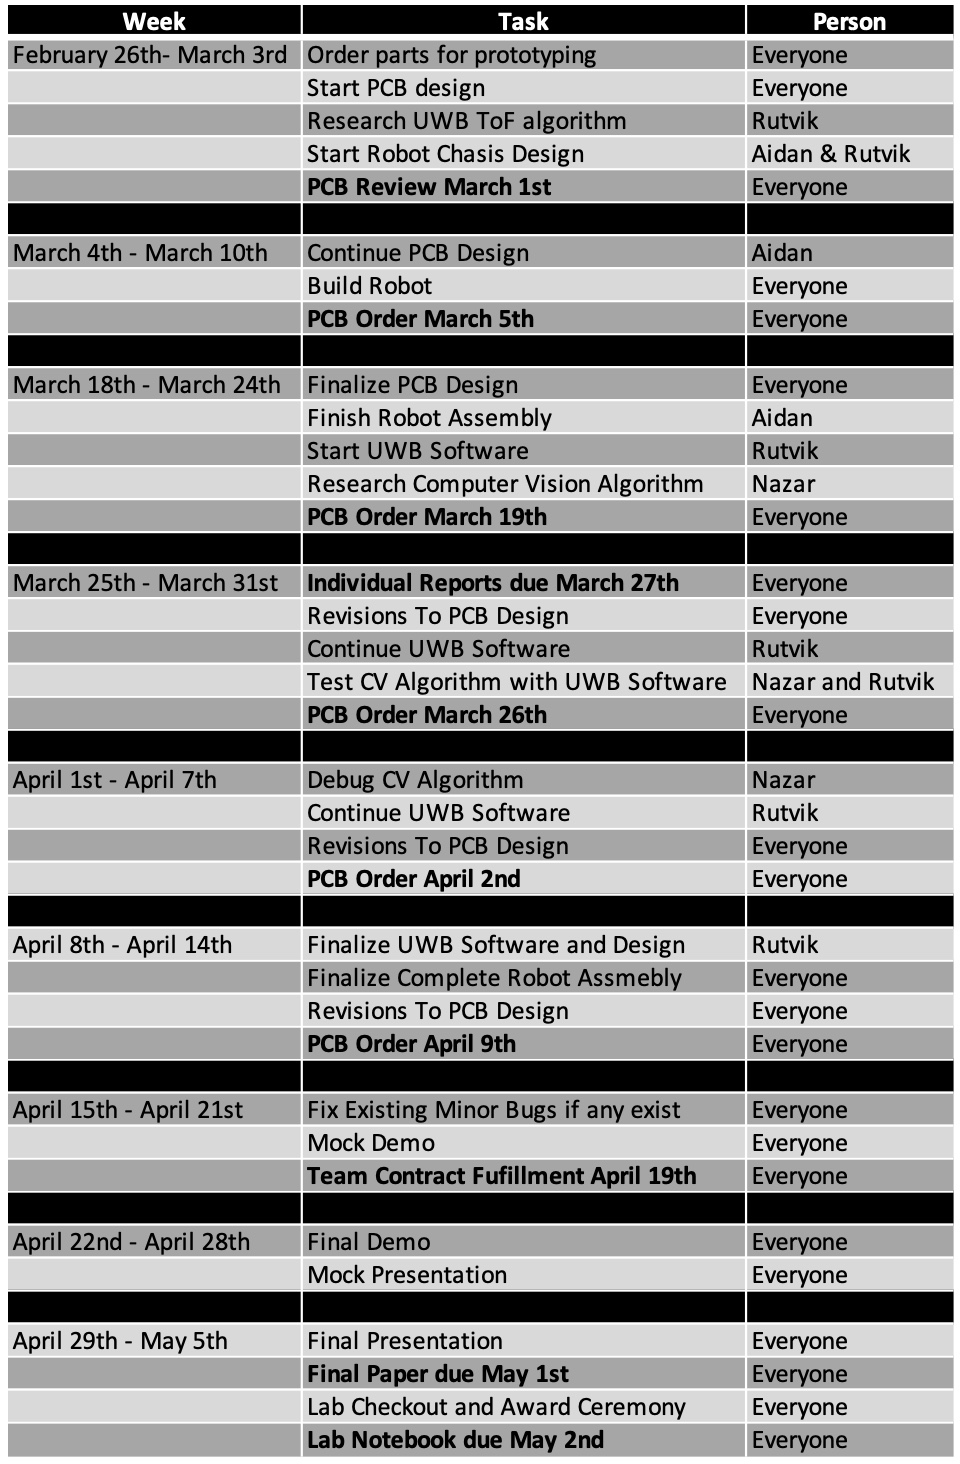
\includegraphics[width=0.7\textwidth]{Schedule.png}\\
    \caption{ Tentative Project Schedule  } 
    \label{fig:Schedule}
\end{center}
\end{figure}

\newpage

\section{Ethics and Safety}
\subsection{Ethical Considerations}
As we continue through the development of our project, we are unwavering in our dedication to abide by the ethical and safety principles outlined by the Association for Computing Machinery (ACM) and the Institute of Electrical and Electronics Engineers (IEEE). As we embark on this project, we pledge our commitment to adhere to these standards, ensuring that our actions and choices uphold the highest level of professionalism and integrity.

As outlined in Section I of the IEEE Code of Ethics, we pledge to “uphold the highest standards of integrity, responsible behavior, and ethical conduct in professional activities” \cite{IEEE_2020}. We will prioritize safety in our design and adhere to ethical design practices. Educating the parents and caregivers about the robot’s use and limitations will allow for informed decision-making. Following relevant laws and regulations regarding this technology will also be a high priority.

In the same Code of Ethics, outlined in Section III, we pledge to “strive to ensure this code is upheld by colleagues and co-workers” \cite{IEEE_2020}. We will support each other in ethical conduct and foster a culture of ethical behavior. Open communication will be established and encouraged to raise concerns and provide guidance to team members.

\subsection{Safety Considerations}
This project aligns with the safety principles outlined in the ACM Code of Ethics and Professional Conduct. Safety remains our number one priority and as outlined in Section 1.2 \cite{ACM_2018}, we will avoid negative consequences, especially when those consequences are significant and unjust. We will take careful consideration of potential impacts and minimize harm. In the context of this project, we will ensure that the robot’s design and operation prioritizes safety, especially to the children this product aims to assist. We will work to analyze potential risk and consider the robot’s mobility and interaction with its environment.

As well as promoting safety, privacy is also a very important guideline that will be followed, which is outlined in Section 1.6. As professionals, we must safeguard the personal information of our users, especially if it involves children. As it relates to this project, we will ensure that no data will be collected and stored in an external location. Data collection will be minimized to only what is necessary for the robot to operate.

One aspect of our project where safety must be considered is regarding the use of lithium batteries. We acknowledge the potential risks associated with the misuse of lithium batteries. We are committed to following the safety guidelines associated with the batteries we plan on using. More specifically, maintaining the battery’s temperature within the recommended range. Also, we are dedicated to the responsible disposal of batteries to ensure sustainability.

Since we are incorporating motors into our design, we will deploy essential control systems to mitigate potential hazards such as collisions with the environment. Safe operation will be ensured with the use of sensors, vision systems, and warning systems.

\newpage

\bibliographystyle{IEEEtran}
\bibliography{ref}

\end{document}
